\documentclass{article}
\usepackage[utf8]{inputenc}
\usepackage{../../utils/personalmacros}

\title{Algorithmics Exercise 3}
\author{Konstantin Mark}
\date{December 2022}

\begin{document}

\maketitle


\listoftheorems[ignoreall,show={exercise}]

\newpage

\begin{exercise}[(MI)LP Modeling]
    Propose (mixed integer) linear programs for each of the following three functions such that the optimal objective value corresponds to $f_j(x_1,x_2), j = 1, 2, 3$. \begin{enumerate}
        \item $f_1(x_1, x_2) = \min \{x_1,x_2\}$ with $0\leq x_i\leq C, i = 1,2$.
        \item $f_2(x_1,x_2) = |x_1 - x_2|$ with $0\leq x_i\leq C, i = 1,2$.
        \item $f_3(x_1,x_2) = x_1\mathrm{XOR} x_2$ with $x_i \in \{0,1\}, i=1,2$.
    \end{enumerate}
    Note: Your solutions need to work for arbitrary choices of $x_1$ and $x_2$. (e.g. enforcing $x_1\leq x_2$ is not allowed).
\end{exercise}

\begin{solving}
    \begin{enumerate}
        \item Assume that $x_1,x_2$ are constant then we model as \begin{align*}
            \max \quad &z\\
            \text{s.t.}\quad& z\leq x_1\\
            & z\leq x_2\\
        \end{align*}  
         Assume that $x_1,x_2$ are variables, then we model as 
         \begin{align*}
            \max\quad& (1,0,0)^T\cdot(z, x_1, x_2)\\
            \text{s.t.}\quad& z\leq x_1\\
            & z\leq x_2\\
            &x_1 \leq C\\
            &x_2\leq C
        \end{align*}  
        \item Assume that $x_1,x_2$ are constant, then we model as \begin{align*}
            \min\quad& z\\
            \text{s.t.}\quad&z\geq x_1-x_2\\
            &z\geq x_2-x_1\\
        \end{align*}
        Assume that $x_1,x_2$ are variables, then we model as \begin{align*}
            \min\quad& z\\
            \text{s.t.}\quad&z\geq x_1-x_2\\
            &z\geq x_2-x_1\\
            &x_1\leq C\\
            &x_2\leq C
        \end{align*}
        \item Assume that $x_1,x_2$ are constant, then we model as \begin{align*}
            \min\quad& z\\
            \text{s.t.}\quad&z\geq x_1-x_2\\
            &z\geq x_2-x_1\\
        \end{align*}
        Assume that $x_1,x_2$ are variables, then we model as \begin{align*}
            \min\quad& B\\
            \text{s.t.}\quad&z\geq x_1-x_2\\
            &z\geq x_2-x_1\\
            &x_1\in \{0,1\}\\
            &x_2\leq \{0,1\}
            \end{align*}
    \end{enumerate}

\end{solving}



\begin{exercise}[LP Modeling]
    Consider a communication network consisting of $n$ nodes which are connected by communication links. Let $A$ be the set of all links. Each link $(i,j)\in A$ allows one-way transmission from node $i$ to node $j$ and can carry up to $u_{ij}$ bits per second. There is a positive charge $c_{ij}$ per bit transmitted along that link. Each node $k$ generates data at the rate of $b^{kl}$ bits per second that have to be transmitted to node $l$, either through a direct link $(k,l)$ or by tracing a sequence of links. The goal is to choose paths along which all data reach their intended destinations, while minimizing the total cost. We allow the data with the same origin and destination to be split and be transmitted along different paths. Formulate this problem as a linear programming problem. Take care that bits reach their correct targets and not just any target!
\end{exercise}
\begin{solving}
    Let $x_{ij}^{kl} \in \mathbb N$ denote the number of bits with origin $k$ and destination $l$ transmitted along $(i,j)$. Then consider the following optimization problem\begin{align}
        \min \qquad & \sum_{(i,j)\in A} c_{ij}\left(\sum_{k,l} x_{ij}^{kl}\right)\\
        \text{s.t.}\qquad & x_{ij}^{kl}\geq 0 &\forall i,j,k,l\in V\\
        &\sum_{k,l}x_{ij}^{kl}\leq u_{ij}& \forall (i,j)\in A\label{2:upp}\\
        & \sum_{j: (k,j)\in A} x_{kj}^{kl} = b^{kl}& \forall k,l\in V \label{2:dest}\\
        & \sum_{i: (i,l)\in A} x_{il}^{kl} = b^{kl}& \forall k,l\in V \label{2:orig}\\
        & \sum_{i: (i,j)\in A} x_{ij}^{kl} = \sum _{m: (i,m)\in A} x_{jm}^{kl} & \forall j,k,l, j\neq k, j\neq l \label{2:flow}
    \end{align}
    Then here \begin{enumerate}
        \item [\eqref{2:upp}] implements the upper bound for each transmission line $(i,j)\in A$,
        \item [\eqref{2:dest}] implements that node $k$ transmits $b^{kl}$ bits with destination $l$ to its neighbors,
        \item [\eqref{2:orig}] implements that node $l$ receives $b^{kl}$ bits with of origin $k$,
        \item [\eqref{2:flow}] implements that bits coming from $k$ with destination $l$ should flow through any $j\neq k, j\neq l$ unhindered.
    \end{enumerate}
\end{solving}

\newpage

\begin{exercise}[LP Feasible Region]
    Draw the feasible region of the following linear program
    \begin{align}
        \max \quad & sx & +& ty\\
        \text{s.t}& -2x&-& y &\geq & -7\\
        &-3x &+&2y &\geq &0\\
        &-x&+&4y&\leq &18\\
        &&&y&\leq &4
    \end{align}

Give appropriate values for $s$ and $t$ such that the linear program has \begin{enumerate}
    \item exactly one optimal solution,
    \item multiple optimal solutions, where each one is bounded, where each one is bounded (i.e., none of its components has an arbitrarily large magnitude),
    \item multiple optimal solutions, unbounded,
    \item no optimal solution
\end{enumerate}
(the problem should not be changed to a feasibility problem)
\end{exercise}
\begin{solving}
    \begin{figure}[H]
        \centering
        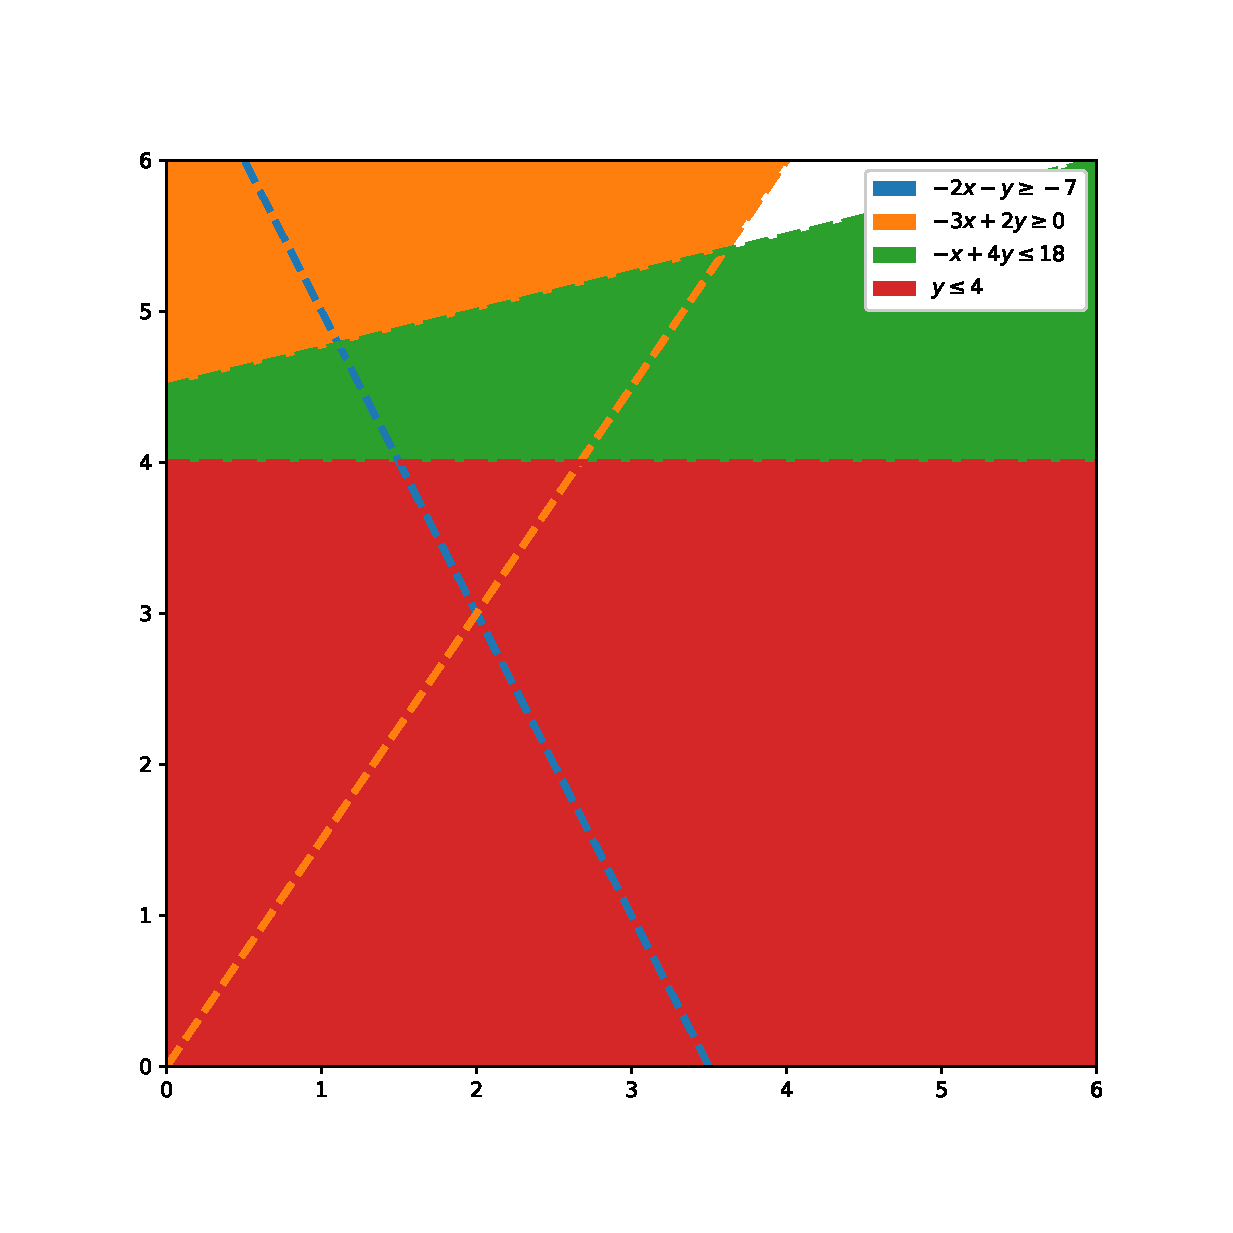
\includegraphics{5/exercise/quick.eps}
        \caption{Caption}
        \label{fig:my_label}
    \end{figure}
\end{solving}


\newpage

\begin{exercise}[LP Duality]
    Given the following primal problem \begin{equation*}
        \begin{array}{crcrcrcr}
             \min & 1.5 x_1 & + & 2x_2 &+ & 4.5x_3\\
             \text{s.t.}&  -x_1 & + & x_2 &+ & x_3 & \geq &2\\
             &  -5x_1 & + & 3x_2 &- & 5x_3 & \leq &15\\
              &  x_1 & + & x_2 &+ & x_3 & = &5\\
              &  &  & x_2 & & & \geq &0\\
              & &  &  & & x_3 & \leq &0\\
        \end{array}
    \end{equation*}
    \begin{enumerate}
        \item Form the corresponding dual problem.
        \item Show by complementary slackness that the primal solution $x = (1.5,5, -1.5)$ is optimal.
    \end{enumerate}
\end{exercise}
\begin{solving}
    \begin{enumerate}
        \item The corresponding dual problem is \begin{equation*}
            \begin{array}{crcrcrcr}
             \max & 2 p_1 & + & 15p_2 &+ & 5p_3\\
             \text{s.t.}&  p_1 & + & 3p_2 &+ & p_3 & \leq &2\\
             &  p_1 & + & -5p_2 &+ & p_3 & \geq &4.5\\
              &  -p_1 & - & 5p_2 &+ & p_3 & = &1.5\\
              & p_1 &  &  & & & \geq &0\\
              & &  &p_2   & & & \leq &0\\
        \end{array}
        \end{equation*}
        by using the rules from the lecture: \begin{figure}[H]
            \centering
            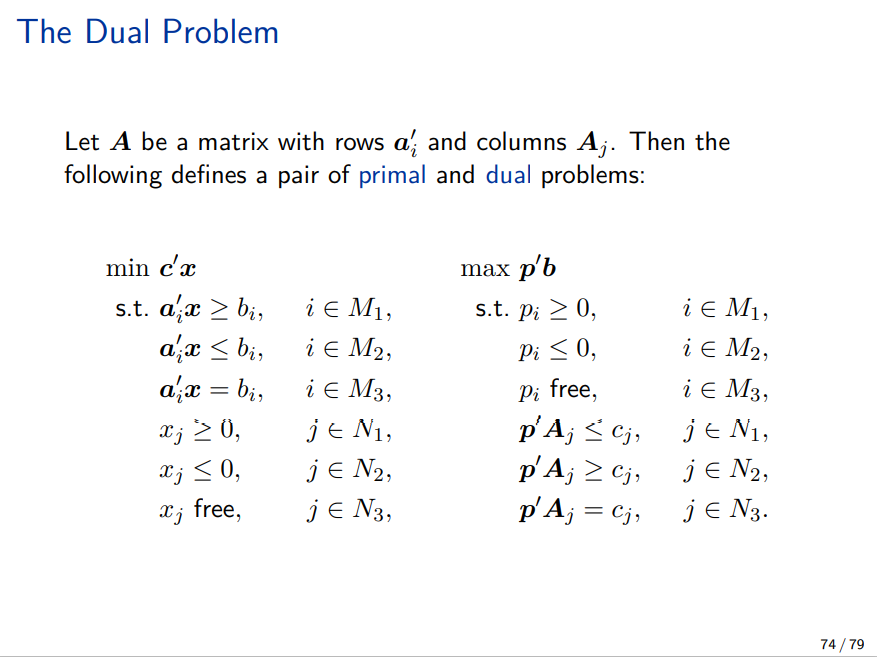
\includegraphics[scale = .5]{5/exercise/dual.png}
            \label{fig:my_label}
        \end{figure}
        \item The theorem of complementary slackness states that feasible solutions $x, p$ to the primal and dual problems are optimal if and only if \begin{equation*}
            p_i(a_i'x - b_i) = 0, (c_j-p'A_j)x_j = 0 \forall i, j
        \end{equation*}
        Note that $x$ is feasible, as \begin{equation*}
        \begin{array}{rcrcrcr}
             
              -x_1 & + & x_2 &+ & x_3 & = 2 \geq &2\\
              -5x_1 & + & 3x_2 &- & 5x_3 & = 15\leq &15\\
               x_1 & + & x_2 &+ & x_3 & = &5\\
               &  & x_2 & & & = 5 \geq &0\\
              &  &  & & x_3 & = -\frac32\leq &0\\
        \end{array}
        \end{equation*}
        This also directly shows $Ax= b$ and thus $a_i'x-b_i = 0$. Solving the linear equation system $pA = c$ gives the solution $(\frac 32, -\frac5{16}, \frac{23}{16})$ which is also feasible in the dual problem and fulfills $c_j-p'A_j = 0$. Thus, both $x$ and $p$ are optimal.
    \end{enumerate}
\end{solving}


\end{document}  